\chapter{Trajectory Generator}\label{chap:trajectory_generator}
We utilize the trajectory planning
approach in [4] to generate thousands of feasible
trajectories per second, and then choose the best one to
follow, with frequent replanning as we follow the trajectory

\section{Base trajectory prediction}

\section{Rapid Trajectory}
how to compute the acceleration...
comparision between diff imu and thrust
\subsubsection{Compute the acceleration}
The Rapid trajectory generator needs an initial and a final state. The initial state is always selected as the current position velocity and acceleration of the quadrotor. From the state estimate of MSF we have the first two information, while we have to compute the acceleration.\\
There are several ways to make this calculation:
\begin{itemize}
\item IMU measurements:
\item finite difference of velocity:
\item total thrust:
\end{itemize}

\begin{figure}[!ht]
    \centering
    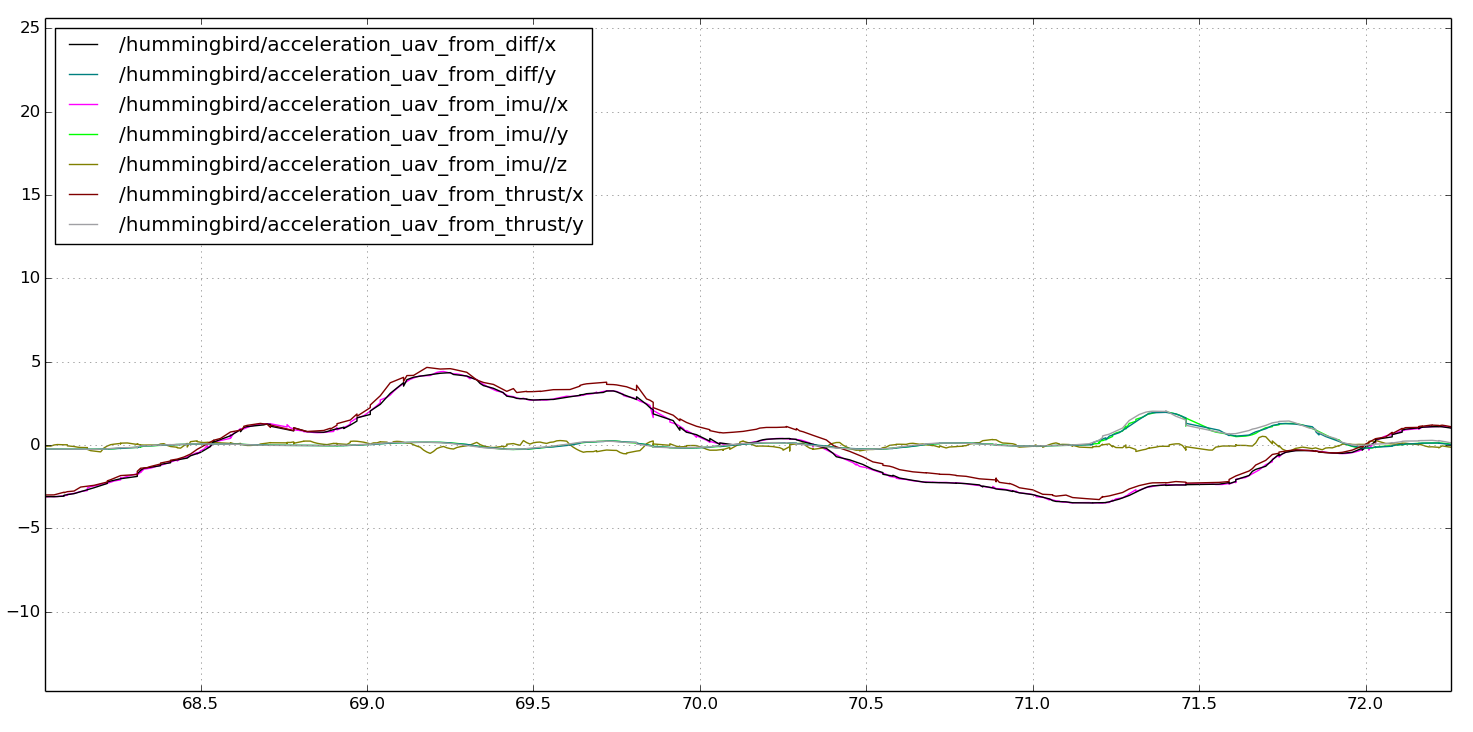
\includegraphics[width=0.97\textwidth]{img/comparison_acc.png}
    \caption{Comparison Acceleration}
    \label{fig:comparison_acc}
\end{figure}

\begin{figure}[!ht]
    \centering
    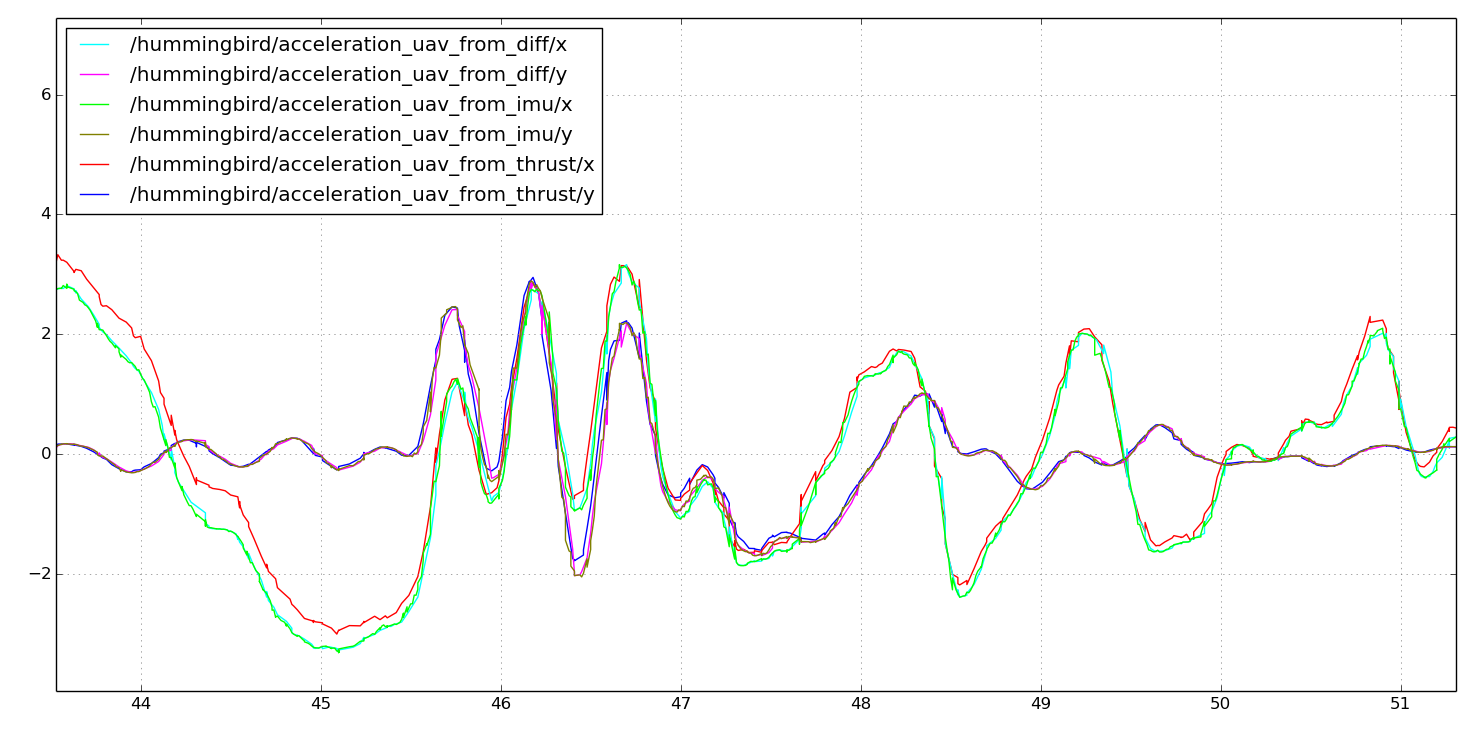
\includegraphics[width=0.97\textwidth]{img/comparison_acc_mass_changed.png}
    \caption{Comparison Acceleration Different Mass}
    \label{fig:comparison_acc_mass_changed}
\end{figure}

\section{Results}
